We wish to design a thermal fin as in Fig. \ref{prj2_thermalfin} to conduct heat from a surface.

\begin{figure*}[h!]
\centering
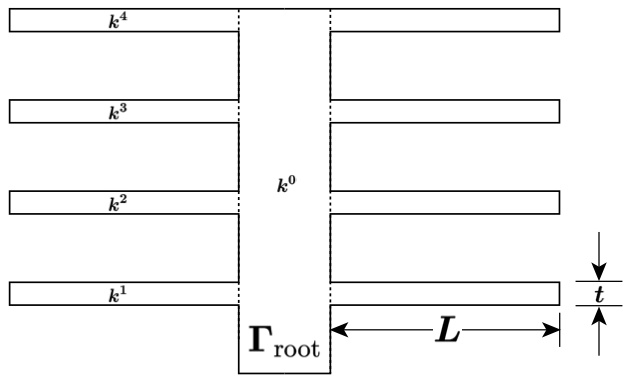
\includegraphics[width=0.5\textwidth]{figures/prj2_thermalfin.png}\\
\caption{Design of the thermal fin, with heat being absorbed at $\Gamma_\text{root}$, conducted up through the post $\Omega^0$ and conducted away by the subfins $\Omega^i$.}
\label{prj2_thermalfin}
\end{figure*}

The parameter space we explore is $\underline{\mu}=\{ k^1,k^2,k^3,k^4,\text{Bi} \}$, where
\begin{itemize}[noitemsep,nolistsep]
    \item $k^0$ is thermal conductivity of the post
    \item $k^i$, the thermal conductivity of the $i$-th subfin, is represented as a multiple of $k_0$
    \item Bi is the Biot number
    \item the post is of width $w=1$ and height $h=4$
    \item the subfins are of thickness $t=0.25$ and length $L=2.5$
\end{itemize}

In the steady state, the temperature distribution within the fin, $u(\underline{\mu})$, is given by
\begin{align}
    -k^i\nabla^2u^i = 0\qquad\text{in}\>\Omega^i,\>i=0,...\>,4
\end{align}

At the boundary intersections $\Gamma_\text{int}^i$ between the domains of the subfins $\Omega_i$ and the central post $\Omega_0$, continuity of temperature and heat-flux must be satisfied.
\begin{align}
    \begin{split}
        u^0 &= u^i \\
        -(\nabla u^0\cdot \hat{\mathbf{n}}^i) &= -k^i(\nabla u^i\cdot \hat{\mathbf{n}}^i)
    \end{split}
    \qquad \text{on}\>\Gamma^i_\text{int},\>i=1,...\>,4
\end{align}

where $\hat{\mathbf{n}}^i$ is the outward normal on $\Gamma^i_\text{int}$.

At the fin root boundary $\Gamma_\text{root}$, we have Neumann flux boundary condition
\begin{align}
    - (\nabla u^0\cdot \hat{\mathbf{n}}^0) &= -1 \qquad \text{on}\>\Gamma^\text{root}
\end{align}

And on the boundaries of $\Omega^i$ exposed to the fluid, $\Gamma_\text{ext}$, we have Robin boundary condition
\begin{align}
    -k^i (\nabla u^i\cdot \hat{\mathbf{n}}^i) &= \text{Bi}\cdot u^i
    \qquad \text{on}\>\Gamma^i_\text{ext},\>i=0,...\>,4
\end{align}
